\documentclass{article}
\usepackage[utf8]{inputenc}
\usepackage[portuguese]{babel}
\usepackage{enumitem}
\usepackage{a4wide}
\usepackage[a4paper, margin=1in]{geometry}
\usepackage{graphicx}
\usepackage{xcolor}
\usepackage{url}
\usepackage{hyperref}
\usepackage[parfill]{parskip}
\usepackage{fancyhdr}

\def\BibTeX{{\rm B\kern-.05em{\sc i\kern-.025em b}\kern-.08em
    T\kern-.1667em\lower.7ex\hbox{E}\kern-.125emX}}
    
\pagestyle{fancy}
\fancyhf{}

\renewcommand{\headrulewidth}{0.03cm}% 2pt header rule
\renewcommand{\headrule}{\hbox to\headwidth{%
  \color{castanho-ue}\leaders\hrule height \headrulewidth\hfill}}
  
\renewcommand{\footrulewidth}{0.03cm}% 2pt header rule
\renewcommand{\footrule}{\hbox to\headwidth{%
  \color{castanho-ue}\leaders\hrule height \headrulewidth\hfill}}
  
\rfoot{\thepage}

\definecolor{castanho-ue}{HTML}{ad4758}

\pagenumbering{roman}
\begin{document}

\begin{titlepage}

\begin{minipage}{0.7\textwidth}
\noindent\LARGE\textbf{Front-end Developer\\\\}
\Large{Licenciatura em Eng. Informática\\}
\large{Estágio-Projeto 2021-2022\\}
\end{minipage}
\begin{minipage}[t]{0.3\textwidth}\raggedleft

\includegraphics[width=.9\linewidth]{images/di.pdf}
\end{minipage}
\noindent
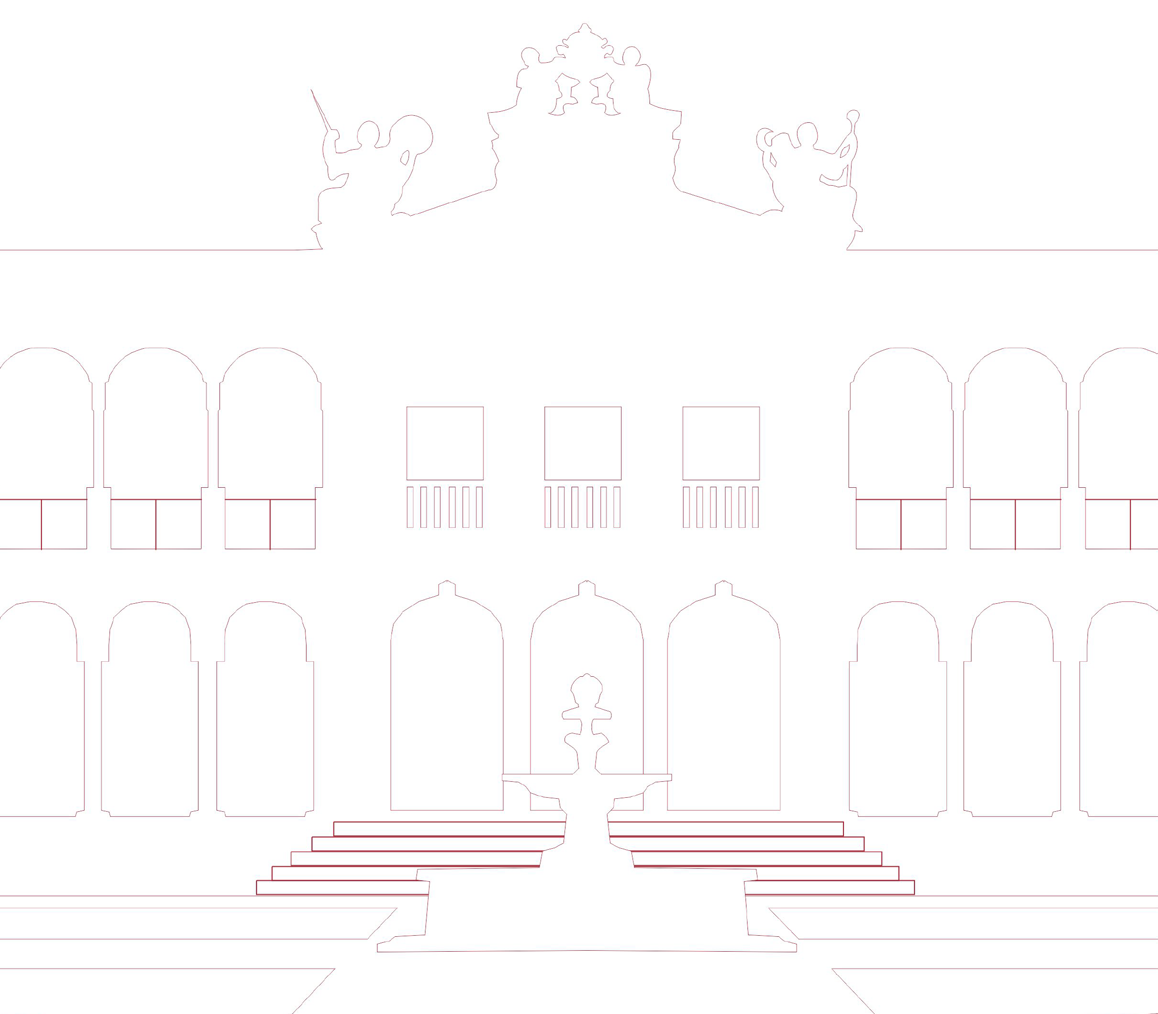
\includegraphics[trim={0 2cm 0 0}, clip,  width=\linewidth]{images/claustros.png}\\

\vspace{0.5cm}
\noindent\textcolor{castanho-ue}{\rule{\textwidth}{0.03cm}}

\vspace{0.5cm}
\noindent\large\textbf{Ricardo Marques Oliveira\\}

\noindent
Orientador na empresa: Fábio Belga\\     
Orientador no departamento: Professor José Saias

\emph{\\Trabalho desenvolvido na empresa Optiply no âmbito da disciplina de Estágio-Projeto da Licenciatura em Eng. Informática.}\\ 

\begin{flushright}
\emph{Évora, \today}
\end{flushright}

\end{titlepage}


\cleardoublepage
\tableofcontents

\cleardoublepage
\pagenumbering{arabic}
\section{Introdução}
\hspace*{0.5cm} Este relatório foi elaborado no âmbito da licenciatura em Engenharia Informática, pertencente ao Departamento de Informática da Escola de Ciências e Tecnologia da Universidade de Évora, pela Unidade Curricular Estágio-Projeto, desempenhado na empresa Optiply. Tem como objetivo a apresentação e descrição de toda a atividade desempenhada, bem como das tecnologias e métodos aplicados no decorrer do estágio. \newline
\hspace*{0.5cm} A educação em contexto laboral, recentemente adotada para a licenciatura em Engenharia Informática, prepara os alunos e proporciona a experiência prática dos conceitos adquiridos no decorrer da formatura, em contexto real no mercado de trabalho propriamente dito. Promove assim, o desenvolvimento de competências, tanto técnicas como organizacionais, cruciais para o futuro. \newline
\hspace*{0.5cm} Em simultâneo, para a instituição que alberga os formandos também retira proveito, uma vez que, facilita os processos de recrutamento de novo pessoal, proporcionando assim também uma constante adaptação à evolução tão constante que existe na área da tecnologia. \newline
\hspace*{0.5cm} O estágio promoveu também, para auxílio mais ativo ao aluno, um orientador na empresa e um orientador no departamento.

\hspace*{0.5cm} As ferramentas utilizadas no decorrer deste período foram Angular \cite{angular, angular-wiki, angular-docs}

Deve incluir as referências que achar serem relevantes no contexto do seu trabalho, na Secção \ref{referencias}. As gestão das conferências deve ser feita usando \BibTeX~\cite{bibtex}. Todas as referências devem ser citadas no texto do relatório, no local apropriado. Pode, por exemplo, fazer as citações como no seguinte parágrafo:

“O sistema foi implementado como um serviço RESTful \cite{richardson2008restful,rodriguez2008restful}, usando o framework Spring Boot \cite{springboot-wikipedia, springboot} para a sua implementação. A autenticação das mensagens é feita através de \emph{hash-based message authentication code} (HMAC) \cite{krawczyk1997hmac, hmac-wikipedia}”

\subsection{Enquadramento}
Descrever resumidamente onde foi realizado o estágio e se estava integrado numa equipa ou não.

\subsection{Objetivos}
Descrever resumidamente onde foi realizado o estágio e se estava integrado numa equipa ou não.

\subsection{Contribuições}
Descrever resumidamente onde foi realizado o estágio e se estava integrado numa equipa ou não.

\subsection{Estrutura do documento}
Descrever resumidamente onde foi realizado o estágio e se estava integrado numa equipa ou não.

\cleardoublepage
\section{Ambiente empresarial}
Diz respeito à natureza da organização onde realizou o estágio, à equipa onde estava inserido e qual a sua posição na equipa. Se for uma grande empresa, esta seção provavelmente será longa; para uma pequena empresa, pode ser bastante curta. Pode, por exemplo, incluir parágrafos como os seguintes:
"A Megalomaniac Enterprises é um conglomerado que opera em mais de 120 países, com a sua sede em Liechtenstein. É uma empresa privada detida e gerida pelo Sr. Aurwen Geldmann. As suas operações variam de mineração a produtos farmacêuticos e de lavanderias a bancos. Existem 37 empresas operacionais distintas dentro do grupo.

Durante o meu ano industrial, fui contratado por uma das subsidiárias bancárias, a Burma Rangoon International Banking Emporium, no seu escritório em Londres perto das Casas do Parlamento. O escritório de Londres tem quatro divisões, três operacionais (banca privada, banca comercial, serviços especiais) e uma divisão de serviços comuns. A divisão de serviços comuns é responsável pelo fornecimento de infraestrutura (por exemplo, computação e telecomunicações) para o resto do escritório. 

Trabalhei no departamento de comunicações da divisão de serviços comuns. No departamento de comunicações existem várias equipas separadas. Inicialmente trabalhei na equipa de manutenção, sendo responsável pela rede local no escritório. Após os primeiros três meses, foi-me oferecida a oportunidade, que aceitei, ser transferido  para a equipa de projectos especiais. Apesar desta equipa reportar ao chefe do escritório de Londres, também, por vezes, recebia instruções diretamente do próprio Sr. Geldmann."


\cleardoublepage
\section{Estado da arte}
Se no âmbito do seu trabalho de estágio fez o levantamento e/ou análise de várias soluções, ferramentas ou metodologias, com o objectivo de escolher a melhor, deve incluir uma descrição desse trabalho nesta secção, incluindo as conclusões a que chegou.
Esta secção pode não fazer sentido em alguns trabalhos.


\cleardoublepage
\section{Ambiente de desenvolvimento}
Nesta secção deve descrever o ambiente de hardware e software onde trabalhou. Isso deve ser razoavelmente abrangente sem ser demasiado detalhado. Pode/deve incluir comentários sobre sua experiência com este ambiente.

\subsection{Ambiente técnico}
\subsubsection{Hardware}
Esta secção pode não fazer sentido em alguns trabalhos.

Pode, por exemplo, incluir parágrafos como os seguintes:

"O computador que recebi para meu próprio uso era uma torre Dell com um processador Intel Core i7 , 8 GB de memória e um disco rígido de 500 GB. Este computador estava ligado a uma rede interna de 100 Mbps com identificação de endereço MAC para acesso interno. A rede estava dividida em duas sub-redes no router, uma para a rede por fios interna e outra para a rede sem fios. A rede foi dividida desta forma para evitar o acesso sem fios a serviços internos sem autenticação. A autenticação pode ser conseguida usando uma VPN para se ligar à rede interna.

A empresa opera um conjunto de servidores locais principalmente da Dell e um da Oracle. Os servidores Dell são usados como SCM (Software Configuration Management),  servidores FTP (File Transfer Protocol) e como servidores web internos. 

Existem dois servidores de controle de versões, um dos quais apenas de acesso interno e o outro com acesso externo. Os servidores suportam CVS, SVN e Git.

Os servidores Dell também contêm aplicações web para navegar nos repositórios. Existe também um servidor Windows, que espelha um servidor em Paris. O servidor da Oracle é usado para virtualização."


\subsubsection{Software}
Nesta secção deve descrever as ferramentas de software que usou no âmbito do seu trabalho de estágio, incluindo qual o seu papel no trabalho realizado.

\subsubsection{Ambiente aplicacional}
Nesta secção deve descrever o contexto aplicacional onde o trabalho realizado se enquadra:

\begin{itemize}
\item Se o seu trabalho fizer parte de um sistema/aplicação maior, deve descrever esse sistema/aplicação, qual o seu papel e como se enquadra. 
\item Se o seu trabalho for “standalone”, então deve descrever o seu ambiente de operação, e, no caso de interagir com outros sistemas, deve descrever essa interação.
\end{itemize}


\subsection{Metodologia de trabalho}
Nesta secção deve descrever a metodologia de trabalho adoptada durante a realização do estágio, devendo incluir:

\begin{itemize}
    
\item Processos desenvolvimento de software usados;
\item Gestão do processo de desenvolvimento;
\item Planificação do trabalho;
\item Interacção com os restantes membros da equipa de trabalho (se existente);

\end{itemize}

\cleardoublepage
\section{Trabalho desenvolvido}
Esta secção deve começar com um resumo claro e bem estruturado. Deve apresentar de forma resumida o trabalho realizado durante o seu estágio. Este resumo deve incluir a lista de tarefas realizadas e timeline respectivo.

Exemplo de um possível resumo:

Quando entrei para a empresa, fui enviado para um curso de formação de quatro semanas para aprender Ruby e como usar as várias ferramentas utilizadas regularmente no departamento. O curso também me apresentou os padrões e procedimentos da empresa.

Após a conclusão do curso, juntei-me à equipa de cinco pessoas responsáveis por manter o sistema de contabilidade de compras. A principal tarefa da equipa naquele momento era modificar o sistema para que os gerentes pudessem fazer consultas on-line sobre ordens de compra pendentes. Recebi dois pequenos programas para escrever e realizar testes unitários. Já existia um projeto detalhado para cada um dos programas: cada um tinha cerca de 200 instruções; escrever e testar os dois demorou cerca de oito semanas.

Fui então convidado a ajudar na produção dos dados de teste para a versão on-line do sistema. Isso envolveu uma leitura cuidadosa da especificação funcional, o que me levou a perceber melhor o que era feito pelo sistema. Esta tarefa demorou cerca de dez semanas para produzir os dados necessários. Os dados de teste foram revistos por outros membros da equipa e levámos mais duas semanas para incorporar as modificações solicitadas.

\subsection{Descrição detalhada}
Nesta secção deve  selecionar e ampliar, em sub-secções separadas, as partes do trabalho desenvolvido no âmbito do seu estágio que lhe parecem mais relevantes e interessantes.

\cleardoublepage
\section{Avaliação crítica}
Nesta secção deve apresentar o que aprendeu com a experiência, evitando ser trivial. Além de discutir o que aprendeu do ponto de vista técnico, deve escrever algo sobre a sua experiência não técnica, em áreas como o trabalho em equipa e a comunicação.

Alguns exemplos de comentários que pode escrever nesta secção:

"Fiquei surpreendido com a extensão dos testes realizados. Eu sabia que os testes eram importantes, mas não tinha percebido que isso significava seguir a especificação funcional e testar cada instrução implementada. Demorou mais tempo para testar um módulo do que  implementá-lo.

Dada a seriedade com que os testes foram realizados, foi estranho descobrir que outras formas de gestão de qualidade eram quase inexistentes. Não existiu uma revisão formal das especificações e não houve revisão do código. Não havia gestão de configuração e ocorreram vários erros porque foram usadas versões erradas de alguns módulos.

Tecnicamente, acho que não aprendi muito com o meu estágio, excepto como programar em Ruby - uma experiência que espero nunca mais repetir. Porém, aprendi muito sobre a forma como as equipas de desenvolvimento de software trabalham e o que significa ter utilizadores reais."


\cleardoublepage
\bibliographystyle{unsrt}
\bibliography{bibs}
\label{referencias}

\end{document}
